Le solide ABCDEFGH est un cube. On se place dans le repère orthonormé $\left(\text{A};\vect{\imath},\,\vect{\jmath},\,\vect{k}\right)$ de l'espace dans lequel les coordonnées des points B, D et E sont : \[\text{B}(3;0;0)\text{, } \text{D} (0;3;0) \text{ et } E(0;0;3).\]
%
\begin{center}
	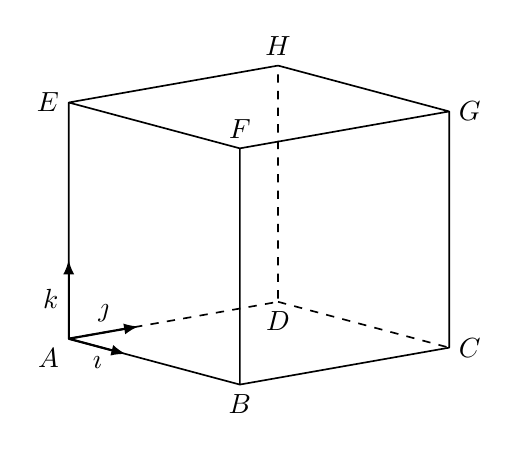
\begin{tikzpicture}[x={(-15:0.75cm)},y={(10:0.9cm)},z={(90:1cm)},line join=bevel]
		\coordinate (A) at (0,0,0) ; \draw (A) node[below left] {$A$} ;
		\coordinate (B) at (3,0,0) ; \draw (B) node[below] {$B$} ;
		\coordinate (C) at (3,3,0) ; \draw (C) node[right] {$C$} ;
		\coordinate (D) at (0,3,0) ; \draw (D) node[below] {$D$} ;
		\coordinate (E) at (0,0,3) ; \draw (E) node[left] {$E$} ;
		\coordinate (F) at (3,0,3) ; \draw (F) node[above] {$F$} ;
		\coordinate (G) at (3,3,3) ; \draw (G) node[right] {$G$} ;
		\coordinate (H) at (0,3,3) ; \draw (H) node[above] {$H$} ;
		\draw[semithick,dashed] (A)--(D)--(H) (D)--(C) ;
		\draw[semithick] (A)--(B)--(F)--(E)--cycle (B)--(C)--(G)--(F) (G)--(H)--(E) ;
		\draw[thick,->,>=latex] (A)--++(1,0,0) node[midway,below] {$\vect{\imath}$} ;
		\draw[thick,->,>=latex] (A)--++(0,1,0) node[midway,above] {$\vect{\jmath}$} ;
		\draw[thick,->,>=latex] (A)--++(0,0,1) node[midway,left] {$\vect{k}$} ;
	\end{tikzpicture}
\end{center}

On considère les points $P(0;0;1)$, $Q(0;2;3)$ et $R(1;0;3)$.

\begin{enumerate}
	\item Placer les points $P$, $Q$ et $R$ sur la figure en \textsf{ANNEXE} qui sera à rendre avec la copie.
	\item Montrer que le triangle $PQR$ est isocèle en $R$.
	\item Justifier que les points $P$, $Q$ et $R$ définissent un plan.
	\item On s'intéresse à présent à la distance entre le point $E$ et le plan $(PQR)$.
	\begin{enumerate}
		\item Montrer que le vecteur $\vect{u}(2;1;- 1)$ est normal au plan $(PQR)$.
		\item En déduire une équation cartésienne du plan $(PQR)$.
		\item Déterminer une représentation paramétrique de la droite $(d)$ passant par le point $E$ et orthogonale au plan $(PQR)$.
		\item Montrer que le point $L\left(\dfrac23;\dfrac13;\dfrac83\right)$ est le projeté orthogonal du point $E$ sur le plan $(PQR)$.
		\item Déterminer la distance entre le point $E$ et le plan $(PQR)$.
	\end{enumerate}
	\item En choisissant le triangle $EQR$ comme base, montrer que le volume du tétraèdre $EPQR$ est $\dfrac23$.
	
	On rappelle que le volume $V$ d'un tétraèdre est donné par la formule : \[V = \dfrac13 \times \text{aire d'une base} \times \text{hauteur correspondante}.\]
	\item Trouver, à l'aide des deux questions précédentes, l'aire du triangle $PQR$.
\end{enumerate}

